

\section{OpticalElement: \textquotedbl{}armazones\textquotedbl{}%
  \label{opticalelement-armazones}%
}

\textbf{Element}: atmosphere

\textbf{Alias}: ATMO

\textbf{Description}: Atmosphere and location details for Cerro Armazones


\subsection{Global properties%
  \label{global-properties}%
}

\begin{quote}
\begin{alltt}
\begin{lstlisting}[frame=single]
    altitude : 3060
   longitude : -70.1918
    latitude : -24.5899
 temperature : 7
    humidity : 0.1
    pressure : 0.755
         pwv : 2.5
     airmass : !OBS.airmass
 pupil_angle : !OBS.pupil_angle
 pixel_scale : !INST.pixel_scale
      season : 0
        time : 0
  background : \{'filter_name': 'Ks', 'value': 13.6, 'unit': 'mag'\}
element_name : armazones
\end{lstlisting}
\end{alltt}
\end{quote}


\subsection{Effects%
  \label{effects}%
}

Summary of Effects included in this optical element:

\setlength{\DUtablewidth}{\linewidth}
\begin{longtable*}[c]{|p{0.120\DUtablewidth}|p{0.384\DUtablewidth}|p{0.189\DUtablewidth}|p{0.108\DUtablewidth}|p{0.154\DUtablewidth}|}
\hline
\textbf{%
element
} & \textbf{%
name
} & \textbf{%
class
} & \textbf{%
included
} & \textbf{%
z\_orders {[}2{]}
} \\
\hline
\endfirsthead
\hline
\textbf{%
element
} & \textbf{%
name
} & \textbf{%
class
} & \textbf{%
included
} & \textbf{%
z\_orders {[}2{]}
} \\
\hline
\endhead
\multicolumn{5}{c}{\hfill ... continued on next page} \\
\endfoot
\endlastfoot

armazones
 & 
armazones\_atmo\_skycalc\_ter\_curve
 & 
SkycalcTERCurve
 & 
True
 & 
112 .. 512
 \\
\hline
\end{longtable*}
\label{tbl-armazones}


\subsubsection{SkycalcTERCurve: \textquotedbl{}armazones\_atmo\_skycalc\_ter\_curve\textquotedbl{}%
  \label{skycalctercurve-armazones-atmo-skycalc-ter-curve}%
}

\textbf{Included by default}: \texttt{True}

\textbf{File Description}: atmospheric spectra pulled from the skycalc server

\textbf{Class Description}: <no docstring>

\textbf{Changes}:

\begin{itemize}
\item \end{itemize}


\paragraph{Data%
  \label{data}%
}

\begin{figure}[H]
\noindent\makebox[\linewidth][c]{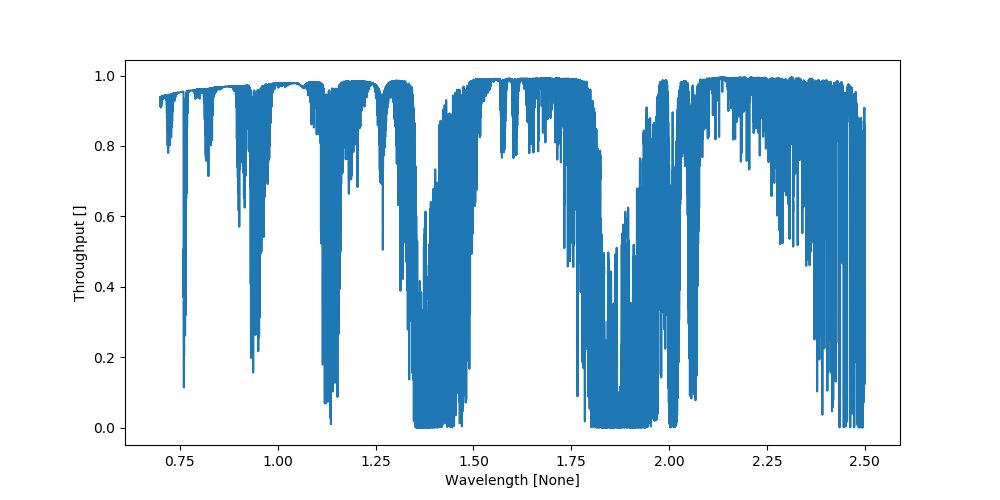
\includegraphics{armazones_atmo_skycalc_ter_curve.png}}\phantomsection\label{fig-armazones-atmo-skycalc-ter-curve}
\end{figure}


\paragraph{Meta-data%
  \label{meta-data}%
}

\begin{quote}
\begin{alltt}
\begin{lstlisting}[frame=single]
            filename : None
                name : armazones_atmo_skycalc_ter_curve
             include : True
            altitude : 3060
           longitude : -70.1918
            latitude : -24.5899
         temperature : 7
            humidity : 0.1
            pressure : 0.755
                 pwv : 2.5
             airmass : 1.2
         pupil_angle : 0
         pixel_scale : 0.004
              season : 0
                time : 0
          background : \{'filter_name': 'Ks', 'value': 13.6, 'unit': 'mag'\}
        element_name : armazones
         observatory : armazones
                wmin : 699.9999999999999
                wmax : 2499.9999999999995
               wunit : um
              wdelta : 0.9999999999999999
    rescale_emission : \{'filter_name': 'Ks', 'filename_format': 'filters/TC_filter_\{\}.dat', 'value': 13.6, 'unit': 'mag'\}
             z_order : [112, 512]
        ignore_wings : False
            wave_min : 0.7
            wave_max : 2.5
           wave_unit : um
            wave_bin : 0.001
 report_plot_include : True
report_table_include : False
              action : transmission
            position : 0
\end{lstlisting}
\end{alltt}
\end{quote}
